\chapter{Aufbau eines Prototypen}
\section{H-Brücke}
Die Brückenschaltung orientiert sich an der Schaltung des zuvor verwendeten Motortreibers sowie an der vorgeschlagenen Schaltung aus dem Datenblatt der Halbbrücken und erlaubt, dass sich der Motor je nach Durchschalten in beide Richtungen drehen kann.
Als Halbbrücken dienen zwei BTN8982 mit jeweils einem p-channel highside MOSFET und einem n-channel lowside MOSFET mit bereits integrierten Schutzmechanismen wie Abschaltung bei zu geringer Spannung oder Übertemperatur beinhalten.  Das Blockdiagramm dieser Halbbrücken ist in nachstehender Abbildung dargestellt.
\begin{figure}[h]
	\centering
		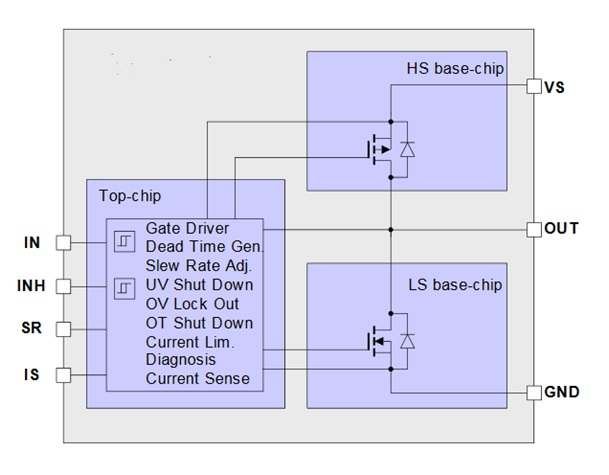
\includegraphics{Bilder/Blockdiagramm Halbbruecken.jpg}
	\caption{Blockdiagramm Halbbrücken}
	\label{fig:Blockdiagramm Halbbruecken}
\end{figure}
In dem Blockdiagramm sind bereits die PINs der Halbbrücken zu erkennen. Diese sollen nun in Tabelle \ref{tab:Pinverteilung} nochmal aufgezählt und ihre Funktionen erklärt werden.

\begin{table}[h]
	\centering
		\begin{tabular}{l|p{5cm}|p{5cm}|p{5cm}}
			Pin Nummer & Bezeichnung & Erläuterung & Anschluss an \\ \hline
			1 & GND (Ground) & & Ground MCU \\
			2 & IN (Input) & definiert die Schalterstellung (1 = High Switch Mode; 0= Low Switch Mode) & Ausgangspin MCU \\
			3 & INH (Inhibit) & 1: Betriebsmodus
0: Schlafmodus & Ausgangspin MCU \\
			4, 8 & OUT (Output) & Ausgang der Brückenschaltung & Aktor \\
			5 & SR (Slew Rate) & & \\
			6 & IS (Status) & & Einganspin MCU\\
			7 & VS (Supply) & & Stromversorgung\\
		\end{tabular}
	\caption{Pinverteilung Halbbrücken}
	\label{tab:Pinverteilung}
\end{table}
Der Status Pin liefert dabei für eine Halbbrücke im High Switch Mode eine zum fließenden Versorgungsstrom proportionale Spannung, für eine Halbbrücke im Low Switch Mode keine Spannung oder Strom und im Fehlbetrieb eine konstante unabhängige Spannung.

Im ersten Entwicklungsschritt wurde die Schaltung auf einem Steckbrett getestet und anstatt des Aktors zwei LEDs in die Brückenschaltung eingebaut. Nachdem diese Schaltung, versorgt durch eine 8 Volt Batterie, mit einem Testskript erfolgreich getestet werden konnte sollte im nächsten Schritt die Brückenschaltung auf eine Lochrasterplatine gelötet werden, die auch bei höheren Strömen beständig sind, damit auch der Motor und die tatsächliche Versorgerspannung angeschlossen werden können. 